\section{Úvod}
    Nedeterministické konečné automaty (NKA) prezentovali Michael Rabin a Dana Scott v \cite{FA_and_Their_Decisin_Problems}. Oproti své deterministické variantě se vyznačují schopností přechodu do více následujících stavů na základě stejného přijatého znak. To umožňuje NKA kompaktněji reprezentovat daný jazyk. Na druhou stranu tato vlastnost působí minimalizaci NKA složitou. I přes obtížnou minimalizaci jsou NKA široce využívány napříč téměř všemi odvětvími počítačové vědy, například při reprezentaci regulárních výrazů, pro monitorování vysokorychlostních sítí \cite{FPGA_based_network_scaning}, v abstraktním regulárním model checkingu \cite{ARMC}, verifikaci programů manipulujícími s řetězci \cite{String_constraints_for_ver} nebo v rozhodovacích procedurách WS1S a WS2S logiky \cite{On_equivalence_checking, Nested_antichains_for_WS1S}. NKA jsou dokonce využívány v bioinformatice pro vyhledávání sekvencí nukleotidových kyselin v DNA \cite{DNA_pattern_analysis_using_FA}.

    Základní technikou snižující nároky na výpočetní zdroje (paměť, čas nebo množství hardwarových komponentů) při práci s NKA je právě minimalizace. Nejznámější technikou minimalizace je slučování stavů \cite{Oldest_Merge,Simulation_based_minimization,On_nfa_reduction}, které vyhledává dva jazykově ekvivalentní stavy a ty následně sloučí v jeden. Dalším přístupem je prořezávaní hran přechodů \cite{Simulation_based_minimization, Lorenzo_prunning_saturation}, které na základě jazykové inkluze dvou stavů odstraní přechod jazykově slabšího stavu, protože má jistotu, že funkce tohoto odstraněného přechodu je již zastoupena jazykově silnějším stavem. Opakem k prořezávání hran přechodů je jejich přidávání (saturace) \cite{Oldest_Merge, Lorenzo_prunning_saturation}, kde právě nově přidané hrany mohou umožnit další slučování stavů nebo odstraňování jiných hran.

    Přestože kombinace zmíněných minimalizačních metod redukuje u většiny automatů jejich velikost až o 50 \%, tak ve výsledných automatech stále existují duplicitní sekvence přechodů. Existují také typy automatů, které nejsou dosavadními postupy vůbec minimalizovatelné. Do této skupiny patří automaty s~lineární strukturou (bez větvení) nebo automaty repre-zentující slova s daným infixem a stejným prefixem i sufixem (např. \textit{abba, cbbc}). V těchto případech nemůže slučování stavů, prořezávání či přidávání přechodů automat nijak minimalizovat. Důvodem je, že tyto redukční přístupy pracují na základě jazykových inkluzí a tyto typy automatů žádnou inkluzi neobsahují. Ve struktuře zmíněných automatů se vyskytují pouze úseky podobných přechodů (např. \textit{bb} z předchozího příkladu).

    Práce popisuje minimalizační algoritmus, který využívá podobné sekvence přechodů k redukci velikosti automatu. Prezentovaná metoda pracuje na základě informovaného převodu nedeterministického konečného automatu na nedeterministický zásobníkový automat (NZA). V NZA lze podobné úseky, nahradit jednou procedurou, která na základě symbolu uložené-ho na zásobníku rozpozná, ve které větvi původního automatu se výpočet nachází. Cílem úspěšného převodu je nahrazení takových sekvencí přechodu, že úspora způsobena jejich redukcí bude převyšovat nad režii zásobnikových operací. Při použití tohoto postupu minimalizace se lze, pro dostatečně velké automaty se slovy obsahujícími stejný prefix a sufix, přiblížit až 100\% redukci velikosti.

    Převod NKA na NZA lze připodobnit k převodu čistě sekvenčního programu na program využívající mezi sebou navzájem komunikující procedury. Podob-ně jako v NZA je i v programu využit zásobník volání pro uložení informace o větvi, ve které se program při volání nachází a kam se má výpočet vrátit po skončení procedury.

\section{Základní pojmy}
    Tato sekce definuje základní teoretické pojmy využívané v minimalizačním algoritmu, jakými jsou nedeterministický konečný automat a nedeterministický zásobníkový automat. A dále zavádí upravenou definici relace simulace, která bere v potaz pouze přechody do vzdálenosti $k \in \mathbb{N}$ od zkoumaného stavu a nerozlišuje mezi koncovými a nekoncovými stavy.

    \subsection{Nedeterministický konečný automat}
        \textit{Nedeterministický konečný automat} (NKA) je pětice $M = (Q, \Sigma, \delta, i, F)$, kde:
        \begin{itemize}
            \item $Q$ je konečná množina stavů,
            \item $\Sigma$ je abeceda,
            \item $\delta : Q \times \Sigma \rightarrow 2^Q$ je přechodová funkce,
            \item $i \in Q$ je počáteční stav a
            \item $F \subseteq Q$ je množina koncových stavů.
        \end{itemize}

        Přechodovou funkci $\delta$ lze také zobecnit pro množi-nu symbolů. Mějme $q \in Q$ a $A \subseteq \Sigma$, pak platí, že $\delta(q, A) = \bigcup_{a\in A} \delta(q, a)$.

        K přechodové funkcí definujeme také inverzní funkci $\delta^{-1}$, kde platí: $q \in \delta^{-1}(r, a) \iff r \in \delta(q, a)$, pro $a \in \Sigma$ a $q, r \in Q$.

        \subsubsection*{Konfigurace}
            \textit{Konfigurace} NKA je uspořádaná dvojice $C \in Q \times \Sigma^*$. $(q, w) \in C$ značí, že se řízení automatu nachází ve stavu $q$ a na vstupu zbývá nezpracovaný řetězec $w$.

        \subsubsection*{Přechod automatu}
            \textit{Přechod automatu} je binární relace $\vdash\, \subseteq C \times C$, která je definována takto: $(q, w) \vdash (r, w') \iff w = aw' \land r \in \delta(q, a)$, pro $q, r \in Q$, $w, w' \in \Sigma^*$, $a \in \Sigma$.

        \subsubsection*{Jazyk}
            \textit{Dopředný jazyk stavu} $q \in Q$ je množina $\overrightarrow L(q) = \{w \in \Sigma^*\, |\, (q, w) \vdash (f, \epsilon)\textnormal{, kde }f \in F\}$.

            \noindent\textit{Zpětný jazyk stavu} $q \in Q$ je množina $\overleftarrow L(q) = \{w \in \Sigma^*\, |\, (i, w) \vdash (q, \epsilon)\}$.

            \noindent\textit{Jazyk automatu} $M$ je množina $L(M) = \overrightarrow L(i)$.

        \subsubsection*{Abeceda stavu}
            Pro NKA dále zaveďme \textit{abecedu stavu}, která je jednoznačně určena funkcí $\sigma : Q \rightarrow 2^\Sigma$, kde platí $a \in \sigma(q) \iff \exists\,r \in Q: r \in \delta(q, a)$, pro $a \in \Sigma$.

    \subsection{Nedeterministický zásobníkový automat}
        \textit{Nedeterministický zásobníkový automat} (NZA) je sedmice $M = (Q, \Sigma_\epsilon, \Gamma_\epsilon, \delta, i, S, F)$, kde:
        \begin{itemize}
            \item $Q$ je konečná množina stavů,
            \item $\Sigma_\epsilon$ je vstupní abeceda\footnote{$\Sigma_\epsilon = \Sigma \cup \{\epsilon\}$},
            \item $\Gamma_\epsilon$ je zásobníková abeceda,
            \item $\delta : Q \times \Sigma_\epsilon \times \Gamma_\epsilon \rightarrow 2^{Q \times \Gamma_\epsilon}$ je přechodová funkce,
            \item $i \in Q$ je počáteční stav,
            \item $Z \in \Gamma$ je počáteční zásobníkový symbol a
            \item $F \subseteq Q$ je množina koncových stavů.
        \end{itemize}

        Podobně jako pro NKA lze definovat přechodovou funkci také pro množinu symbolů $A \subseteq \Sigma$, nebo $B \subseteq \Gamma_\epsilon$.

        Pro inverzní přechodovou funkci $\delta^{-1}$ v NZA platí: $(q, \beta) \in \delta^{-1}(r, a, \gamma) \iff (r, \gamma) \in \delta(q, a, \beta)$, kde $q,r \in Q$, $a \in \Sigma_\epsilon$, $\beta, \gamma \in \Gamma_\epsilon$. Povšimněte si, že u inverzní funkce se zamění vkládaný a vyjímaný zásobníkový symbol.

        \subsubsection*{Konfigurace}
            \textit{Konfigurace} NZA je uspořádaná trojice $C \in Q \times \Sigma^* \times \Gamma^*$. $(q, w, \beta) \in C$ značí, že se řízení automatu nachází ve stavu $q$, na vstupu zbývá nezpracovaný řetězec $w$ a zásobník obsahuje řetězec $\beta$ (vrchol zásobníku je vlevo).

        \subsubsection*{Přechod automatu}
            \textit{Přechod automatu} je binární relace $\vdash\, \subseteq C \times C$, která je definována takto: $(q, w, \beta) \vdash (r, w', \beta') \iff w = aw' \land \beta = X\alpha \land \beta' = Y\alpha \land (r, Y) \in \delta(q, a, X)$, pro $q, r \in Q$, $w, w' \in \Sigma^*$, $a \in \Sigma_\epsilon$, $X, Y \in \Gamma_\epsilon$.

        % \subsubsection*{Abeceda přechodu}
        %     \textit{Abeceda přechodu} je určena funkcí $\sigma : Q \times Q \rightarrow 2^\Sigma$, kde platí $a \in \sigma(q, p) \iff \exists\, \beta \in \Gamma : p \in \delta(q, a, \beta)$.

        % \subsubsection*{Push abeceda}
        %     \textit{Push abeceda} stavu je určena funkcí $\gamma_{push} : Q \rightarrow 2^{\Gamma^*}$, kde platí $\beta \in \gamma_{push}(q) \iff \exists\, p \in Q\; \exists\, a \in \Sigma : p \in \delta(q, a, \beta)$. Push abecedy stavu $q \in Q$ je tedy množina všech $\beta \in \Gamma^*$, které jsou vloženy na zásobníky při výstupních přechodech stavu $q$.

        % \subsubsection*{Pop abeceda}
        %     \textit{Pop abeceda} stavu je určena funkcí $\gamma_{pop} : Q \rightarrow 2^{\Gamma^*}$, kde platí $\beta \in \gamma_{pop}(q) \iff \exists\,p \in Q\; \exists\, a \in \Sigma : q \in \delta(p, a, \beta)$. Lze vidět, že po abeceda stavu $q \in Q$ je definována obdobně jako push abeceda. Jedná se o množinu všech $\beta \in \Gamma^*$, které jsou vyjmuty ze zásobníku při přechodu do stavu $q$.

    \subsection{Simulace}
        Pro popis vztahu mezi stavy s podobnou sekvencí přechodů je použita modifikovaná \textit{relace simulace} \cite{Computing_simulaitons, When_simulation_meets_antichains}. Oproti původní relaci zkoumá modifikovaná relace simulace (\textit{k-aproxsim}) pouze přechody do vzdálenosti $k \in \mathbb{N}$ od zkoumaného stavu. Dále \textit{k-aproxsim} nerozlišuje mezi koncovými a nekoncovými stavy.

        \subsubsection*{Simulace}
            \textit{Simulace} na NKA $M$ je kvaziuspořádání $\preceq\, \subseteq Q \times Q$. Nechť $a \in \Sigma$. Relace $p \preceq q$ existuje pouze tehdy, když paltí $r \in F \implies q \in F$ a pro každé $r' \in \delta(r, a)$ existuje $q' \in \delta(q, a)$, pro které dále musí platit $r' \preceq q'$.

        \subsubsection*{K-aproxsim}
            \textit{K-aproxsim} na NKA $M$ je kvaziuspořádání $\precapprox_k\, \subseteq Q \times Q$, pro které platí: pokud je $k = 0$, pak $\precapprox_0 = Q \times Q$, jinak, $r \precapprox_{k} q \iff \forall\, r' \in \delta(r, a)\;\exists\, q' \in \delta(q, a): r' \precapprox_{k-1} q'$, kde $a \in \Sigma$.

\section{Minimalizační techniky}
    Tato sekce uvádí v současnosti nejpoužívanější minimalizační metody, jakými jsou: slučování stavů, pro-řezávání přechodů a přidávání přechodů.

    \subsection{Slučování stavů}
        Dva stavy $p$ a $q$ mohou být sloučeny v jeden, pokud je splněna alespoň jedna z následujících podmínek:
        \begin{itemize}
            \item $\overleftarrow{L}(p) \subseteq \overleftarrow{L}(q) \land \overleftarrow{L}(q) \subseteq \overleftarrow{L}(p)$,
            \item $\overrightarrow{L}(p) \subseteq \overrightarrow{L}(q) \land \overrightarrow{L}(q) \subseteq \overrightarrow{L}(p)$, nebo
            \item $\overleftarrow{L}(p) \subseteq \overleftarrow{L}(q) \land \overrightarrow{L}(p) \subseteq \overrightarrow{L}(q)$.
        \end{itemize}

    \subsection{Prořezávání přechodů}
        Přechod $pa \rightarrow q$\footnote{Namísto $q \in \delta(p, a)$ můžeme psát $pa \rightarrow q$.} může být odstraněn, pokud je splněna jedna z následujících podmínek:
        \begin{itemize}
            \item $\exists\, ra\rightarrow q \land \overrightarrow{L}(p) \subseteq \overrightarrow{L}(q)$
            \item $\exists\, qa\rightarrow p \land \overleftarrow{L}(r) \subseteq \overleftarrow{L}(q)$ nebo
            \item $\exists\, r'a\rightarrow p' \land \overleftarrow{L}(r) \subseteq \overleftarrow{L}(r') \land \overrightarrow{L}(p) \subseteq \overrightarrow{L}(p')$.
        \end{itemize}

    \subsection{Přidávání přechodů}
        Základní myšlenka přidávání přechodů (nebo-li saturace) je analogií k prořezávání přechodů. Přechod $pa \rightarrow q$ může být do automatu přidán pokud je splněna alespoň jedna z následujících podmínek:
        \begin{itemize}
            \item $\exists\, qa\rightarrow r \land \overleftarrow{L}(p) \subseteq \overleftarrow{L}(q)$ nebo
            \item $\exists\, pa\rightarrow q \land \overrightarrow{L}(r) \subseteq \overrightarrow{L}(q)$.
        \end{itemize}

    \subsection{Limitace}
        Lze vidět, že všechny minimalizační techniky jsou založeny na jazykových inkluzích (mohou být určeny na základě simulace). Pak v případě lineárních automatů (bez větvení), nebo automatů slov se stejným prefixem a sufixem nemohou být tyto metody plně využity, protože v těchto automatech existuje minimum stavů v~netriviální jazykové inkluzi.

        \begin{figure}[h]
            \centering
            \captionsetup{justification=justified}
            \begin{tikzpicture}[node distance=1.7cm, every node/.style={font=\footnotesize}]
              \node[state, initial, minimum size=0.5cm] (s) {$s$};
              \node[state, above right of=s, minimum size=0.5cm] (q1) {$q_1$};
              \node[state, below right of=s, minimum size=0.5cm] (q2) {$q_2$};
              \node[state, right of=q1, minimum size=0.5cm] (q3) {$q_3$};
              \node[state, right of=q3, minimum size=0.5cm] (q5) {$q_5$};
              \node[state, right of=q2, minimum size=0.5cm] (q4) {$q_4$};
              \node[state, right of=q4, minimum size=0.5cm] (q6) {$q_6$};
              \node[state, accepting, below right of=q5, minimum size=0.5cm] (f) {$f$};

            \path[->]
                      (s) edge[above left] node{$x$} (q1)
                      (s) edge[below left] node{$y$} (q2)
                      (q1) edge[above] node{$a$} (q3)
                      (q3) edge[above] node{$b$} (q5)
                      (q2) edge[below] node{$a$} (q4)
                      (q4) edge[below] node{$b$} (q6)
                      (q5) edge[above right] node{$x$} (f)
                      (q6) edge[below right] node{$y$} (f);
            \end{tikzpicture}
            \caption{Příklad automatu přijímajícího slovo s~infixem $ab$, a kde prefix i sufix musí být $x$ nebo $y$.}
            \label{sufprefAtm}
          \end{figure}

          Z obrázku \ref{sufprefAtm} lze vidět, že v automatu nelze provést žádnou minimalizaci založenou na jazykových inklu-zích (až na triviální se zde žádné nevyskytují). Přesto si lze všimnout, že se infixová část slova (zbytečně) opakuje. Hlavní motivací práce je fakt, že se v automatech tohoto a podobných typů vyskytují dlouhé opakující se sekvence přechodů, které by mohly být reprezentovány pouze jednou. V dostatečně velkých automatech, obsahujících dlouhé podobné sekvence přechodu, může tato náhrada za jednu proceduru přinést redukci velikosti přechodové funkce blížící se limitně až 100~\%.

\section{Převod NKA na NZA}
    Převod původního NKA na NZA s procedurami sestává z pěti částí. Nejdříve je spočítaná $asim_n$ pro $n = 1,\dots,k$, kde $p \in asim_n(q) \iff q \precapprox_n p$. ($asim_n$ je spočítaná také pro reverzní automat. Pokud se při iteraci redukčního algoritmu vybere prvek z reverzní $asim_n$, pak je redukce prováděná na reverzním automatu.) Pro původní automat je vytvořen odpovídající NZA. Pro všechny stavy z nejsilnější $asim_k(p)$ a~jejich následníky do vzdálenosti $k$ je vytvořena procedura, na kterou se původní stavy přemapují. Všechny přemapované stavy jsou následně odstraněny z automatu i z $asim_n$ pro $n = 1,\dots,k$. Znovu je vybraná nejsilnější $asim_k(p)$. Pokud je $asim_k = \emptyset$, pak se pokra-čuje s $asim_{k-1}$. Po provedení všech přemapování je zjednodušena zásobníková abeceda pomocí \textit{$\alpha$-redukce} a množství přechodů je sníženo \textit{$\epsilon$-redukcí}.

    \subsection{Výpočet $asim_k$}
    Relace $asim_k \subseteq Q \times 2^Q$ pro $k \in \mathbb{N}$ je definována následovně: $p \in asim_k(q) \iff q \precapprox_k p$. Pro výpočet je využit modifikovaný algoritmus RefinedSimilarity \cite{Computing_simulaitons}. Před uvedením algoritmu definujme množinu předchůdců stavů $S \subseteq Q$ jako $anc(S) = \bigcup_{q \in S} \delta^{-1}(q, \Sigma)$. Dále definujme pomocnou relaci $prevasim_k$, kde mno-žina $prevasim(q) \supseteq asim_k(q)$ je množina předpokládaných kandidátů pro $asim_k(q)$.

        \begin{algorithm}[h]
            \scriptsize
            \DontPrintSemicolon
            \setcounter{AlgoLine}{0}
            \KwIn{NKA $M = (Q, \Sigma, \delta, i, F)$, $k \in \mathbb{N}$}
            \KwOut{$asim_k(q)$}

            \vspace{0.2cm}

            \ForAll(){$q \in Q$}
            {
                $asim^1_k(q) = \{r \in Q\, |\, \sigma(q) \subseteq \sigma(r)\}$\;
                \tcc{$\sigma(q)$ je abeceda stavu $q$}
            }
            $prevasim^1_k$ = $Q \times \{Q\}$\;

            \vspace{0.2cm}
            $i = 1$\;
            \While(){$i \leq k$}
            {
                $asim^i_k = asim^{i-1}_k$\;
                \ForAll{$q \in Q$}
                {
                    \ForAll(){$a \in \sigma(q)$}
                    {
                        $s\_by\_a = \{s \in Q\, |\, \exists\, r \in Q: r \in \delta(q, a)\}$\;
                        $acn\_pasim = anc(prevasim^{i-1}_k \cap\, s\_by\_a,\, a)$\;
                        $anc\_asim = anc(asim^{i-1}_k \cap\, s\_by\_a,\, a)$\;
                        $remove = anc\_pasim \setminus anc\_asim$\;
                        \ForAll(){$s \in \delta^{-1}(q, a)$}
                        {
                            $asim^i_k(s) = asim^i_k(s) \setminus remove$\;
                        }
                    }
                }
                $prevasim^i_k = asim^{i-1}_k$\;
                $i = i + 1$\;
            }

            \Return{$asim^k_k$}\;

            \normalsize
            \caption{Výpočet $asim_k$}
            \label{aproxSim-Alg}
        \end{algorithm}

    V první smyčce for algoritmus inicializuje relaci $asim^1_k$, která odpovídá $\precapprox_1$. Oproti původnímu algoritmu počítajícího simulaci zde není rozlišováno mezi koncovými a nekoncovými stavy. Základní myšlenkou algoritmu je, že s každou další iterací cyklu while se vzdálenost na kterou působí relace $asim_k$ prodlužuje, dokud nedosáhne požadované vzdálenosti $k$.

    \subsection{Reprezentace NKA pomocí NZA}
        Před zahájením vyhledávání procedur je původní NKA přepsán do tvaru NZA bez jakékoliv změny vnitřní struktury.

        Mějme dán NKA $M = (Q, \Sigma, \delta, i, F)$. Automat $M$ převedeme na NZA $Z = (Q, \Sigma, \{\bot\}, \delta' , \{\bot\},i, F)$, kde $(p, \epsilon) \in \delta'(q, a, \epsilon) \iff p \in \delta(q, a)$, kde $p, q \in Q$, $a \in \Sigma$.

    \subsection{Vytvoření procedury}
        Mějme dán NZA $Z = (Q, \Sigma, \Gamma, \delta, i, S, F)$ a původní NKA $M = (Q_M, \Sigma_M, \delta_M , I_M, F_M)$. Definujme bijekci $cname : Q \rightarrow Q$, kde $cname(q) = r$ udává, že se stav $q$ přemapoval na stav $r$. $cname$ je inicializován jako identita.

        Procedury se vytváří postupně od nejsilnější dvojice $ (p, S) \in asim_k$, kde $p \in Q$ se nazývá \textit{primární stav} a $(S \setminus \{p\}) \subseteq Q$ množina \textit{sekundárních stavů}. Nejprve je vytvořena \textit{kostra procedury} na základě množiny $follow_k(p) \subseteq Q$, která obsahuje následníky primárního stavu $p$ v automatu $M$ do vzdálenosti $k$. Následně jsou pro každý sekundární stav $s \in (S \setminus \{q\})$ přemapovány všechny stavy z $follow_k(s)$ na tuto kostru.

        \subsubsection*{Stavy do vzdálenosti $k$}
            Množina stavů do vzdálenosti $k \in \mathbb{N}$ od stavu $q \in Q_M$ je definována jako $follow_k(q) = \{s \in Q_M\, |\, (q, w) \vdash^n (s, w'),\; 0 \leq n \leq k,\; w, w' \in \Sigma^*_M\}$.

        \subsubsection*{Síla relace $aim_k(q)$}
            Síla relace $pow(aim_k(q)) \in \mathbb{N}$ je definována následovně: $pow(aim_k(q)) = |\{(r, a, s) \,|\, s \in \delta_M (r, a),\; r, s \in follow_k(q),\; a \in \Sigma_M\}|$.

        \begin{algorithm}[h]
            \scriptsize
            \DontPrintSemicolon
            \setcounter{AlgoLine}{0}
            \KwIn{NZA $Z = (Q, \Sigma, \Gamma, \delta, i, S, F)$, $p \in Q$, $follow_k(p)$, $cname$}
            \KwOut{NZA $Z' = (Q', \Sigma, \Gamma', \delta', i, S, F)$, $cname'$}

            \vspace{0.2cm}
            $follow = follow_k(p) \cap Q$\;
            $Q' = Q$\;
            $\Gamma' = \Gamma \cup follow$\;
            $\delta' = \delta$\;
            \vspace{0.2cm}

            $cname' = cname$\;
            \ForAll(){$q \in follow_k(p)$}
            {
                $t = newState()$ \tcp*{$t \notin Q'$}
                $Q' = Q' \cup \{t\}$\;
                $cname'(q) = t$\;
            }

            \vspace{0.2cm}

            \ForAll(){$q \in follow$}
            {
                $inside = \{(r, a) |\, (r, \beta) \in \delta(q, a, \Gamma), r \in follow\}$\;
                \ForAll(){$(r, a) \in inside$}
                {
                    $\delta' = \delta' \cup \{(cname(q), a, q) \rightarrow (cname(r), r)\}$\;
                }

                $in = \{(r, a, \beta) |\, (r, \beta) \in \delta^{-1}(q, a, \Gamma), r \in Q \setminus follow\}$\;
                \ForAll(){$(r, a, \beta) \in trans\_in$}
                {
                    $\delta' = \delta' \cup \{(r, a, \beta) \rightarrow (cname(q), q)\}$\;
                }

                $out = \{(r, a, \beta) |\, (r, \beta) \in \delta(q, a, \Gamma), r \in Q \setminus follow\}$\;
                \ForAll(){$(p, a, \beta) \in out$}
                {
                    $\delta' = \delta' \cup \{(cname(q), a, q) \rightarrow (r, \beta)\}$\;
                }
            }

            \Return{$Z', cname'$}

            \normalsize
            \caption{Vytvoření kostry procedury}
            \label{mapPrim-Alg}
        \end{algorithm}

        Pro vytvoření kostry procedury stavu $p \in Q$ do vzdálenosti $k \in \mathbb{N}$ je zapotřebí pro každý stav $r \in follow_k(p)$ vygenerovat nový, na který se stav $r$ pře-mapuje. Odpovídající dvojice stavů obsahuje zobrazení $cname$. Přechody vstupující do stavu $cname(r)$ vkládají na zásobník znak $r$ a přechody vycházející ze stavu $cname(r)$ vyjímají ze zásobníků symbol $r$. Lze vidět, že při přechodu ze stavu $r_1 \in follow_k(p)$ do stavu $r_2 \in follow_k(p)$ bude znak $r_1$ vyjmut ze zásobníku a~$r_2$ na zásobník vložen.

        \begin{algorithm}[h]
            \scriptsize
            \DontPrintSemicolon
            \setcounter{AlgoLine}{0}
            \KwIn{NZA $Z = (Q, \Sigma, \Gamma, \delta, i, S, F)$, $follow_k(s)$, $k \in \mathbb{N}$, $cname$}
            \KwOut{NZA $Z' = (Q, \Sigma, \Gamma', \delta', i, S, F)$, $cname'$}

            \vspace{0.2cm}
            $follow = follow_k(s) \cap Q$\;
            $\Gamma' = \Gamma$\;
            $\delta' = \delta$\;
            $cname' = cname$\;
            \vspace{0.2cm}

            $mapped = \emptyset$\;
            $queue = \{(p, s, k, \textbf{False})\}$\tcp*{fronta}
            \While(){$queue \neq \emptyset$}
            {
                $(p, s, i, visible) = queue.pop()$\;
                \If(){$s \in mapped$}
                {
                    \textbf{continue}\;
                }

                \If(\tcp*[f]{s nikdo nemapoval}){$s = cname(s)$}
                {
                    $visible = \textbf{True}$\;
                    $cname'(s) = cname'(p)$\;
                    $\Gamma' = \Gamma' \cup \{s\}$\;
                }
                $mapped = mapped \cup \{s\}$\;

                \vspace{0.2cm}

                \If(){$visible \land i > 0$}
                {
                    \tcc{s nikdo nemapoval. Existuje následník v proceduře.}
                    $inside = \{(r, a, \beta) |\, (r, \beta) \in \delta(s, a, \Gamma), r \in follow\}$\;
                    \ForAll(){$(q, a, \beta) \in inside$}
                    {
                        \eIf(){$r = cname(r)$}
                        {
                            $\delta' = \delta' \cup \{(cname(s), a, s) \rightarrow (cname(r), r)\}$\;
                        }()
                        {
                            $\delta' = \delta' \cup \{(cname(s), a, s) \rightarrow (cname(r), \beta)\}$\;
                        }
                    }

                    $in = \{(r, a, \beta) |\, (r, \beta) \in \delta^{-1}(s, a, \gamma), r \in Q \setminus follow\}$\;
                    \ForAll(){$(r, a, \beta) \in in$}
                    {
                        $\delta' = \delta' \cup \{(r, a, \beta) \rightarrow (cname(s), s)\}$\;
                    }

                    $out = \{(r, a, \beta) |\, (r, \beta) \in \delta(s, a, \gamma), r \in Q \setminus follow\}$\;
                    \ForAll(){$(r, a, \beta) \in out$}
                    {
                        $\delta' = \delta' \cup \{(cname(s), a, s) \rightarrow (r, \beta)\}$\;
                    }
                }

                \vspace{0.2cm}

                \If(){$i > 0$}
                {
                    \tcc{Zařaď do fronty dvojice ekvivalentních následníků.}
                    $next = \{(r, a) |\, (r, \beta) \in \delta(s, a, \gamma), r \in follow\}$\;
                    \ForAll(){$(r, a) \in next$}
                    {
                        \If(){$visible \land r \neq cname(r)$}
                        {
                            \textbf{continue}\;
                        }

                        \If(){$\delta'(p, a, \Gamma) \cap asim_{i-1}(q) = \emptyset$}
                        {
                            \textbf{continue}\;
                        }

                        $next\_p = pick\_one(\delta'(p, a, \Gamma) \cap asim_{i-1}(q))$\;
                        $queue = queue.put(r, next\_p, visible, i-1)$\;

                    }
                }

            }
            \Return{$Z', cname'$}

            \normalsize
            \caption{Mapování sekundárních stavů}
            \label{mapSec-Alg}
        \end{algorithm}

        Mapování větve sekundárního stavu $s \in Q$ je oproti vytváření kostry komplikovanější. Buď primární stav $prim$, pak může nastat situace, že pro dva různé sekun-dární stavy $r_1, r_2 \in asim_k(prim)$, mají jejich množiny následníků $follow_k(r_1)$ a $follow_k(r_2)$ neprázdný prů-nik. Tedy může existovat stav, který je zahrnut ve více než jedné mapované sekvenci. Duplicitní mapování jednoho stavu může vést ke zvýšení počtu přechodů automatu, a proto není povoleno.

        Procedura využívá čtveřice $(p, s, i, visible)$, kde $p \in follow_k(prim)$ je stav z primární větve a stav $s \in follow_k(r)$ je jemu odpovídající stav ze sekundární, kde $s \in asim_i(p)$. Kladná hodnota $i$ udává aktuální výšku zanoření v sekundární větvi. Pokud hodnota $i$ klesne na $0$, mapování se zastaví. Informaci, zda stav $s$ nebyl doposud přemapován nese proměnná $visible \in \{\textbf{True}, \textbf{False}\}$. Pokud již byl počátek sekundární větve přemapován v rámci jiné sekvence, zůstává $visible = \textbf{False}$ a žádné mapování se pro dvojici stavů $s, p$ neprovádí. V opačném případě je mapování podobné vytváření kostry procedury: přemapují se vnitřní (mezi stavy procedury), vstupní (vstupující do stavů procedury) a výstupní (vystupující ze stavů procedury) přechody. Po přemapování dvojice stavů $s, p$ jsou do fronty dvojic dalších stavů zařazeny stavy $s'$, $p'$, kde $s' \in follow_k(r)$ a $p' \in follow_k(prim)$. Pokud již stav $s$ nemá následníky, pak není dvojice $s', p'$ generovaná, jinak $s' \in \delta(s, a, \Gamma)$, $p' \in \delta(p, a, \Gamma)$, $s' \in asim_{i-1}(p')$.

    \subsection{Počáteční stav a symbol na zásobníku}
        Pokud je počáteční stav původního automatu přemapo-ván do procedury (bude následně smazán), musí být ustanoven nový počáteční stav a s ním i zásobníkový symbol. Mějme NZA $Z = (Q, \Sigma, \Gamma, \delta, i, S, F)$ a bijektivní zobrazení $cname$, které je výsledkem mapova-cího algoritmu. Pak automat s novým počátečním symbolem je NZA $Z' = (Q, \Sigma, \Gamma \cup \{i\}, \delta, cname(i), i, F)$.

    \subsection{Koncové stavy}
        Při mapování koncových stavů je zapotřebí řešit podob-ný problém jako u mapování počátečních stavů. Zde však existují dva přístupy. Buď jsou pomocí epsilon přechodů svedeny všechny koncové stavy do jednoho centrálního koncového stavu, nebo bude automat přijímat přechodem do koncového stavu a zároveň na zásobníku musí být symbol daný relací s koncovým stavem. V implementovaném algoritmu je využit druhý přístup.

        \subsubsection*{Centrální koncový stav}
            Mějme NZA $Z = (Q, \Sigma, \Gamma, \delta, i, S, F)$ a bijektivní zobrazení $cname$, které je výsledkem mapovacího algoritmu. Pak automat s centrálním koncovým stavem je NZA $Z' = (Q', \Sigma, \Gamma, \delta', i, S, \{fin\})$, kde $Q' = Q \cup \{fin\} \land fin \notin Q$,

            \vspace{-0.5cm}
            $$
            \delta'(p, a, \beta) =
            \begin{cases}
                \delta(p, a, \beta) \hspace{0.7cm} p \notin F \lor cname(p) \neq p,\\
                \delta(p, a, \beta) \cup \{(fin, \epsilon)\} \hspace{0.7cm} \textit{jinak}.
            \end{cases}
            $$

        \subsubsection*{Koncový stav a koncový symbol}
            Mějme NZA $Z = (Q, \Sigma, \Gamma, \delta, i, S, F)$ a bijektivní zobrazení $cname$, které je výsledkem mapovacího algoritmu. Pak automat přijímající v koncovém stavu se symbolem definovaným relací $\Phi \subseteq F \times \Gamma$ je osmice $Z' = (Q, \Sigma, \Gamma, \delta, i, S, F, \Phi)$, kde:

            \vspace{-0.5cm}
            $$\Phi(f) =
            \begin{cases}
                S & cname(f) = f,\\
                cname(f) & jinak.
            \end{cases}
            $$

            Jazyk automatu $Z'$ je  $L(Z') = \{w \in \Sigma^*\,|\,(i, w, Z) \vdash^* (f, \epsilon, \Phi(f)),\textit{ kde } f \in F\}$.

    \subsection{$\alpha$-redukce}
        Po provedení všech možných přemapování může být velikost zásobníkové abecedy rovna počtu stavů původního automatu. Její velikost je možné snížit $\alpha$-redukcí popsanou algoritmem \ref{betaReduction-Alg}.

        \begin{algorithm}[h]
            \scriptsize
            \DontPrintSemicolon
            \setcounter{AlgoLine}{0}
            \KwIn{NZA $Z = (Q, \Sigma, \Gamma, \delta , i, F)$}
            \KwOut{NZA $rename \subseteq \Gamma \times \Gamma$}

            \vspace{0.2cm}
            $rename = \{(\beta, \beta) | \beta \in \Gamma\}$\;

            $stack = I$\tcp*{zásobník}
            $close = \emptyset$\;

            \While(){$stack \neq \emptyset$}
            {
                $s = stack.pop()$\;
                \If(){$s \in close$}
                {
                    \textbf{continue}\;
                }
                $close = closed \cup \{s\}$\;
                $pop\_in\_by\_push = \{(\gamma, \beta) |\, (q, \gamma) \in \delta^{-1}(s, \Sigma, \gamma)\}$\;
                $pops\_out = \{\beta |\, (q, \gamma) \in \delta(s, \Sigma, \beta)\}$\;

                \ForAll(){$pop \in pops\_out$}
                {
                    $push\_in = pop$\;
                    $pops\_in = \bigcup_{\beta \in pop\_in\_by\_push(pop)} rename(\beta)$\;
                    $pops\_out = \bigcup_{\beta \in pops\_out(pop)} rename(\beta)$\;
                    \If(){$rename(pop) \in pops\_in$}
                    {
                        \textbf{continue}\;
                    }

                    $possible = pops\_in \setminus pops\_out$\;
                    \If(){$possible \neq \emptyset$}
                    {
                        $rename(rename(pop)) = pict\_one(possible)$\;
                    }
                }

                $stack = stack \cup succ(s)$\;

            }
            \Return{$rename$}\;


            \normalsize
            \caption{$\alpha$-redukce}
            \label{betaReduction-Alg}
        \end{algorithm}

        Symbol na zásobníku rozlišuje, ve kterém stavu původního NKA se výpočet nachází. Je zřejmé, že pokud není využito zanořování procedur, pak dvě procedury, které na sebe nenavazují přímo mohou sdílet část zásobníkové abecedy. Místo využívání zásobníku k rozlišování stavů, můžeme také použít zásobník pouze k rozlišování, ve které větvi původního NKA se výpočet nachází. Toto zjednodušení významně ovlivní velikost použité zásobníkové abecedy.

        Pro správnou funkci algoritmu \ref{betaReduction-Alg} musí být ve vstupním NZA použit každý zásobníkový symbol pouze s~jedním stavem (to je zajištěno korektním mapováním). V průběhu algoritmu platí, že pokud byl symbol $\beta \in \Gamma$ vložen na zásobník na vstupním přechodu do stavu $q \in Q$, pak musí být také vyjmut na alespoň jednom přechodu vycházejícím ze stavu $q$. Algoritmus prostupuje automatem do šířky a provádí substituci zásobníkových symbolů. Substituce $\alpha \in \Gamma$ za $\beta \in \Gamma$ u stavu $q \in Q$ je validní, pokud není symbol $\beta$ vyjímán ze zásobníku na žádné výstupní hraně stavu $q$ (může být vkládán).

        \begin{figure}[h]
            \centering
            \captionsetup{justification=justified}
            \begin{tikzpicture}[node distance=3cm, every node/.style={font=\footnotesize}]
              \node[state, minimum size=0.5cm] (q1) {$q_1$};
              \node[state, right of=q1, minimum size=0.5cm] (q2) {$q_2$};
              \node[state, right of=q2, minimum size=0.5cm] (q3) {$q_3$};
              \node[state, below=1cm of q1, minimum size=0.5cm] (r1) {$q_1$};
              \node[state, right of=r1, minimum size=0.5cm] (r2) {$q_2$};
              \node[state, right of=r2, minimum size=0.5cm] (r3) {$q_3$};

            \path[->]
            (q1) edge[below] node{$a,1/2$} (q2)
            (q2) edge[below] node{$b,2/3$} (q3)
            (q2) edge[above, bend right] node{$c,2/1$} (q1)
            (r1) edge[above] node{$a,1/1$} (r2)
            (r2) edge[above] node{$b,1/3$} (r3)
            (r2) edge[below, bend left] node{$c,1/1$} (r1);
            \end{tikzpicture}
            \caption{Příklad validní $\alpha$-redukce na části NZA. Vrchní automat je před a spodní po $\alpha$-redukci. Byla provedena substituce zásobníkového symbolu $2$ za $1$ (pro odlišení jsou symboly celá čísla).}
            \label{betaOkAtm}
          \end{figure}

          \vspace{-1cm}

          \begin{figure}[h]
            \centering
            \captionsetup{justification=justified}
            \begin{tikzpicture}[node distance=3cm, every node/.style={font=\footnotesize}]
              \node[state, minimum size=0.5cm] (q1) {$q_1$};
              \node[state, right of=q1, minimum size=0.5cm] (q2) {$q_2$};
              \node[state, right of=q2, minimum size=0.5cm] (q3) {$q_3$};
              \node[state, below=1cm of q1, minimum size=0.5cm] (r1) {$q_1$};
              \node[state, right of=r1, minimum size=0.5cm] (r2) {$q_2$};
              \node[state, right of=r2, minimum size=0.5cm] (r3) {$q_3$};

            \path[->]
                      (q1) edge[below] node{$a,1/2$} (q2)
                      (q1) -- node[below] {$x,6/6$}  ++(2.65,-0.5cm)
                      (q1) -- node[below] {$y,6/1$}  ++(2.75,+2.6cm)
                      (q2) edge[above] node{$b,2/3$} (q3)
                      (q2) edge[above, bend right] node{$c,2/1$} (q1)
                      (r1) edge[above] node{$a,6/2$} (r2)
                      (r1) -- node[below] {$y,6/6$}  ++(2.65,-1.5cm)
                      (r1) -- node[below] {$x,6/6$}  ++(2.7,+1.5cm)
                      (r2) edge[below] node{$b,2/3$} (r3)
                      (r2) edge[below, bend left] node{$c,2/6$} (r1);
            \end{tikzpicture}
            \caption{Příklad nevalidní $\alpha$-redukce na části NZA. Vrchní část automatu je před a spodní po $\alpha$-redukci. Byla provedena substituce zásobníkového symbolu $1$ za $6$ (pro odlišení jsou symboly celá čísla). Tato substituce změnila jazyk. Nyní je ve spodní části automatu možné provést sekvenci přechodů $(q_2, yx, 2) \vdash (q_1, x, 6) \vdash (q_2, \epsilon, 6)$, která v původní verzi nebyla možná.}
            \label{betaErrAtm}
          \end{figure}

    \subsection{$\epsilon$-redukce}
        Po provedení všech přemapování a $\alpha$-redukce je velikost přechodové funkce $\delta$ rovna velikosti přechodové funkci původního NKA. Hlavním cílem redukčního algoritmu je právě snížení velikosti přechodové funkce. Snížení počtu přechodů mezi stavy $q$ a $r$ využívajících symbol $a \in \Sigma$ lze docílit náhradou přechodů $\{(q, a, \beta) \rightarrow (r, \beta)\,|\, (r, \beta) \in \delta(q, a, \beta),\textnormal{ kde } \beta \in \Gamma\}$ za $\{(q, a, \epsilon) \rightarrow (r, \epsilon)\,|\, (r, \beta) \in \delta(q, a, \beta),\textnormal{ kde } \beta \in \Gamma\}$. Pro validní $\epsilon$-redukci, musí platit rovnost množin symbolů $\{\beta \in \Gamma\,|\, (r, \beta) \in \delta(q, a, \beta)\} = \{\beta \in \Gamma\,|\, (r, \gamma) \in \delta(q, \Sigma, \beta)\}$, jinak nelze $\epsilon$-redukce pro vybrané stavy uskutečnit, protože by došlo ke změně jazyka.

        \begin{figure*}[h]
            \centering
            \captionsetup{justification=justified}
            \begin{tikzpicture}[node distance=2cm, every node/.style={font=\footnotesize}]
                \node[state, initial, minimum size=0.5cm] (q0) {$q_0$};
                \node[state, above right of=q0, minimum size=0.5cm] (q1) {$q_1$};
                \node[state, right of=q1, minimum size=0.5cm] (q2) {$q_2$};
                \node[state, right of=q2, minimum size=0.5cm] (q3) {$q_3$};
                \node[state, right of=q3, minimum size=0.5cm] (q4) {$q_4$};
                \node[state, right of=q4, minimum size=0.5cm] (q5) {$q_5$};
                \node[state, accepting, below right of=q5, minimum size=0.5cm] (q6) {$q_6$};
                \node[state, above of=q2, minimum size=0.5cm] (q7) {$q_7$};
                \node[state, below right of=q0, minimum size=0.5cm] (q8) {$q_8$};
                \node[state, right of=q8, minimum size=0.5cm] (q9) {$q_9$};
                \node[state, right of=q9, minimum size=0.5cm] (q10) {$q_{10}$};
                \node[state, right of=q10, minimum size=0.5cm] (q11) {$q_{11}$};
                \node[state, right of=q11, minimum size=0.5cm] (q12) {$q_{12}$};
                \node[state, below of=q11, minimum size=0.5cm] (q13) {$q_{13}$};
                \node[state, right of=q13, minimum size=0.5cm] (q14) {$q_{14}$};

                \node[state, initial, below=7cm of q0, minimum size=0.5cm] (r0) {$q_0$};
                \node[state, right of=r0, minimum size=0.5cm] (r1) {$p_1$};
                \node[state, right of=r1, minimum size=0.5cm] (r2) {$p_2$};
                \node[state, right of=r2, minimum size=0.5cm] (r3) {$p_3$};
                \node[state, right of=r3, minimum size=0.5cm] (r4) {$p_4$};
                \node[state, right of=r4, minimum size=0.5cm] (r5) {$p_5$};
                \node[state, below of=r2, minimum size=0.5cm] (r6) {$p_6$};
                \node[state, accepting, right of=r5, minimum size=0.5cm] (r7) {$q_{6}$};

                \path[->]
                      (q0) edge[above left] node{$x$} (q1)
                      (q1) edge[above] node{$a$} (q2)
                      (q2) edge[above] node{$b$} (q3)
                      (q3) edge[above right, bend right=45] node{$k$} (q7)
                      (q7) edge[above left, bend right=45] node{$m$} (q1)
                      (q3) edge[above] node{$c$} (q4)
                      (q4) edge[above] node{$d$} (q5)
                      (q5) edge[right, bend left] node{$s$} (q6)
                      (q0) edge[below left] node{$y$} (q8)
                      (q8) edge[below] node{$a$} (q9)
                      (q9) edge[below] node{$b$} (q10)
                      (q10) edge[below] node{$c$} (q11)
                      (q10) edge[below left, bend right] node{$k$} (q13)
                      (q11) edge[below] node{$d$} (q12)
                      (q13) edge[below] node{$m$} (q14)
                      (q12) edge[below, bend right] node{$t$} (q6)
                      (q14) edge[below right, bend right] node{$u$} (q6)

                      (r0) -- node[above] {$\bot$} ++(-0.95, -0.1cm)
                      (r0) edge[above] node{$x,\epsilon/q_1$} (r1)
                      (r0) -- node[above] {$y,\epsilon/q_8$} ++(1.65, 0.6cm)
                      (r1) edge[above] node{$a,q_8/q_8$} (r2)
                      (r1) -- node[above] {$a,q_1/q_1$} ++(1.65, 0.6cm)
                      (r1) edge[below, bend left=70] node{$u,q_{14}/\epsilon$} (r7)
                      (r2) edge[above] node{$b,\epsilon/\epsilon$} (r3)
                      (r3) edge[above] node{$c, \epsilon/\epsilon$} (r4)
                      (r4) edge[above] node{$d, \epsilon/\epsilon$} (r5)
                      (r5) edge[above] node{$s,q_1/\epsilon$} (r7)
                      (r5) -- node[above] {$t,q_8/\epsilon$} ++(1.65, -0.9cm)
                      (r3) edge[below right, bend left=45] node{$k,\epsilon/\epsilon$} (r6)
                      (r6) edge[below left, bend left=45] node{$m, q_8/q_{14}$} (r1)
                      (r6) -- node[above] {$m,q_1/q_1$} ++(-4.3, 0.5cm);

            \end{tikzpicture}
            \caption{Příklad převodu NKA $M$ (nahoře) na NZA $Z$ (dole). Převod byl uskutečněn pomocí uvedených algoritmů (mapování stavů, $\alpha$-redukce a $\epsilon$-redukce). Tento převod využívající vyhledávání procedur ušetřil 7 stavů a 4 přechody při použití pouhých 3 zásobníkových symbolů ($\bot$ se nepočítá).}
            \label{epsilonErrAtm}
          \end{figure*}

        \begin{figure}[h]
            \centering
            \captionsetup{justification=justified}
            \begin{tikzpicture}[node distance=3cm, every node/.style={font=\footnotesize}]
              \node[state, minimum size=0.5cm] (q1) {$q_1$};
              \node[state, right of=q1, minimum size=0.5cm] (q3) {$q_3$};
              \node[state, above=0.5cm of q3, minimum size=0.5cm] (q2) {$q_2$};
              \node[state, below=1cm of q1, minimum size=0.5cm] (r1) {$q_1$};
              \node[state, right of=r1, minimum size=0.5cm] (r2) {$q_2$};
              \node[state, below=0.5cm of r2, minimum size=0.5cm] (r3) {$q_3$};

            \path[->]
                      (q1) edge[above] node{$a,1/1$} (q2)
                      (q1) -- node[above] {$a,2/2$}  ++(2.65,+1.7cm)
                      (q1) -- node[above] {$a,3/3$}  ++(2.68,+2.35cm)
                      (q1) edge[below] node{$b,3/4$} (q3)
                      (r1) edge[above] node{$a,\epsilon/\epsilon$} (r2)
                      (r1) edge[below] node{$b,3/4$} (r3);
            \end{tikzpicture}
            \caption{Příklad validní $\epsilon$-redukce na části NZA. Vrchní část automatu je před a spodní po $\epsilon$-redukci.}
            \label{epsilonOkAtm}
          \end{figure}

          \begin{figure}[h]
            \centering
            \captionsetup{justification=justified}
            \begin{tikzpicture}[node distance=3cm, every node/.style={font=\footnotesize}]
                \node[state, minimum size=0.5cm] (q1) {$q_1$};
                \node[state, right of=q1, minimum size=0.5cm] (q3) {$q_3$};
                \node[state, above=0.5cm of q3, minimum size=0.5cm] (q2) {$q_2$};
                \node[state, below=1cm of q1, minimum size=0.5cm] (r1) {$q_1$};
                \node[state, right of=r1, minimum size=0.5cm] (r2) {$q_2$};
                \node[state, below=0.5cm of r2, minimum size=0.5cm] (r3) {$q_3$};

                \path[->]
                        (q1) edge[above] node{$a,1/1$} (q2)
                        (q1) -- node[above] {$a,2/2$}  ++(2.65,+1.7cm)
                        (q1) -- node[above] {$a,3/3$}  ++(2.68,+2.35cm)
                        (q1) edge[below] node{$b,4/5$} (q3)
                        (r1) edge[above] node{$a,\epsilon/\epsilon$} (r2)
                        (r1) edge[below] node{$b,4/5$} (r3);
            \end{tikzpicture}
            \caption{Příklad nevalidní $\epsilon$-redukce na části NZA. Vrchní část automatu je před a spodní po $\epsilon$-redukci. Chybná $\epsilon$-redukce umožňuje ve spodní části automatu provést přechod $(q_1, a, 4) \vdash (q_2, \epsilon, 4)$, který není v~původní variantě možný.}
            \label{epsilonErrAtm}
          \end{figure}

~\newpage~\newpage

\section{Experimentální výsledky}
    Efektivnost redukčního algoritmu byla testována na automatech reprezentujících jazyk $\{pwp\,|\, \forall\,p \in P\; \forall\, w \in W: W \subseteq \Sigma^* \land P \subseteq \Sigma\}$. Cílem redukce bylo převést NKA na NZA tak, aby byl každý infix $w$ reprezentován pouze jednou, a tím minimalizovat velikost přechodové funkce.

    \subsection{Generování testových automatů}
    \begin{algorithm}[h]
        \scriptsize
        \DontPrintSemicolon
        \setcounter{AlgoLine}{0}
        \KwIn{$alphabet\_cnt, depth, in\_cnt, sections \in \mathbb{N}$, $fork\_p, loop\_p, out\_p \in \langle 0, 1\rangle \subset \mathbb{Q}$}
        \KwOut{NKA $M = (Q, \Sigma, \delta, i, F)$}

        \vspace{0.2cm}

        $\Sigma = \{a \cdot n\, |\, 1 \leq n \leq alphabet\_cnt\}$\;
        $i = init$, $F = \{fin\}$, $Q = F \cup \{i\}$, $\delta = \emptyset$, $trans = \emptyset$\;
        $states = \{1, \dots, in\_cnt\}$, $states\_cnt = in\_cnt$, $reused = \emptyset$\;

        $open^0 = states$\;
        $d = 0$\;
        $branches = 1$\;
        \While(){$d < depth$}
        {
            $open^{d+1} = \emptyset$\;
            \ForAll(){$src \in open^d$}
            {
                \While(){\textnormal{\textbf{True}}}
                {
                    \eIf(){$rand(\langle 0, 1\rangle) < loop\_p$}
                    {
                        $dst = rand(Q)$\;
                        $reused = reused \cup \{state\}$\;
                    }()
                    {
                        $states\_cnt = states\_cnt + 1$\;
                        $dst = states\_cnt$\;
                        $states = states \cup \{dst\}$\;
                        \If(){$rand(\langle 0, 1\rangle) < out\_p$}
                        {
                            $states\_out = states\_out \cup \{dst\}$
                        }
                    }
                    $open^{d+1} = open^{d+1} \cup \{dst\}$\;
                    $trans = trans \cup \{(src, rand(\Sigma), dst)\}$\;

                    \If(){$src \in reused \lor rand(\langle 0, 1\rangle) > fork\_p$}
                    {
                        \textbf{break}
                    }
                    \If(){$((depth - d)*(branches + 1)*sections) + states\_cnt > 800/sections$}
                    {
                        \textbf{break}\tcp*{brání explozi stavů}
                    }
                }
            }
            $d = d + 1$\;
        }
        $states\_out = states\_out \cup open^{d}$\;
        $used\_l = \emptyset$\;
        \ForAll(){$i \in \{0,\dots,sections\}$}
        {
            $l = rand(\Sigma \setminus used\_l)$\;
            $used\_l = used\_l \cup \{l\}$\;
            $\delta = \delta \cup \{(init, l) \rightarrow (q+i*states\_cnt)\,|\, q \in states\_in\}$\;
            $\delta = \delta \cup \{((q+i*states\_cnt), l) \rightarrow fin\,|\, q \in states\_out\}$\;
            $\delta = \delta \cup \{((q+i*states\_cnt), a) \rightarrow (r+i*states\_cnt)\,|$\\\hspace{1.07cm}$\, (q, a, r) \in trans \}$\;
            $Q = Q \cup \{(q+i*states\_cnt)\,|\, q \in states\}$\;
        }

        \Return{$M$}\;

        \normalsize
        \caption{Generátor NKA}
        \label{NKAgen-Alg}
    \end{algorithm}

    Algoritmus \ref{NKAgen-Alg} generuje NKA s $k \in \mathbb{N}$ identickými sekcemi. Vstupní a výstupní hrany jedné sekce obsahují stejný znak, který je unikátní pro každou sekci. Generování lza řídit pomocí parametrů, kde: velikost abecedy automatu značí $aplhabet\_cnt$, $sections$ určuje kolik sekcí bude vytvořeno, $depth$ udává hloubku jednotlivých sekcí, $in\_cnt$ je počet stavů v každé sekci, do kterých vede hrana z počátečního stavu automatu. V každém kroku generování nového stavu je rozhodnuto, zda z aktuálního stavu povede hrana do: konco-vého stavu (s pravděpodobností $out\_p$), do $k$ odlišných stavů (s~pravděpodobností $fork\_p^{k-1}$) nebo do již vytvořeného stavu (s pravděpodobností $loop\_p$).

    \subsection{Výsledky testů}
        Minimalizační algoritmus využívající vyhledávání procedur a převod na NZA byl testován na 960 automatech (s pěti sekcemi) vygenerovaných pomocí algoritmu \ref{NKAgen-Alg}.

        Míra redukce velikosti přechodové funkce auto-matu je zobrazena s použitím houslových grafů. Každý houslový graf je výsledkem minimalizace 20 automatů. Velikost abecedy poloviny automatů je 8 a druhé 16 znaků. Algoritmus byl testován na automatech s hloub-kami sekvencí 5, 10, 20 a 70 pro čtyři různé kombinace parametrů $fork\_p$, $loop\_p$, $in\_cnt$ a $out\_p$.

        Každá testovací sada automatů s danou hloubkou sekvence byla minimalizovaná za použití $asim_1$ (mod-rá), $asim_5$ (červená) a $asim_{10}$ (zelená). Jak již bylo dříve zmíněno, tak pro minimalizaci s $asim_5$ jsou nej-prve použity všechny relace z $asim_5$, poté z $asim_4$ až $asim_1$ (obdobně pro $asim_{10}$).

        Pokud by byly všechny sekce nahrazeny pouze jednou společnou procedurou, pak by minimalizace dosáhla optimální velikosti. Nechť $t$ je celkový počet přechodů, $f$ je počet přechodů vedoucích do koncového stavu a $s$ je počet přechodů vedoucích z počáteč-ního stavu, poté je optimální redukce (v grafu znázorněna zelenou tečkovanou čárou) dána vzorcem:
        $$
        \frac{\frac{t-f-s}{w}+f+s}{t}
        $$

        \begin{figure}[h]
            \centering
            \captionsetup{justification=justified}
            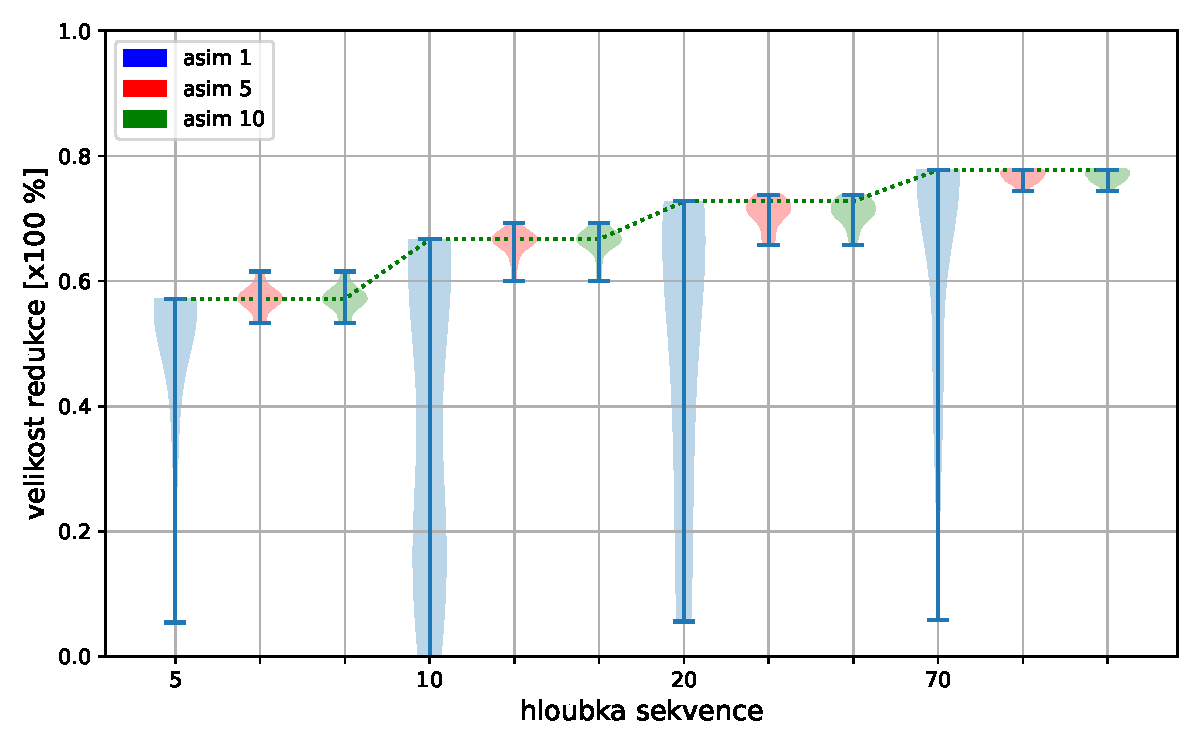
\includegraphics[width=1\linewidth]{5 words: Fork:0.1.pdf}
            \caption{Graf výsledků minimalizace přechodové funkce automatů s následující konfigurací: $in\_cnt = 1$, $fork\_p = 0.1$, $loop\_p = 0$, $out\_p = 0$.}
            \label{res1}
        \end{figure}


        Z obrázku \ref{res1}, a také z ostatních výsledků, je patrné, že využívání $asim_1$ přináší neoptimální výsledky. Tato neoptimálnost redukce je způsobena vytvářením procedur uvnitř jednotlivých sekcí, namísto mezi sekcemi. Relace $asim_1$ využívá pouze přechody do vzdálenosti 1 od zkoumaných stavů což způsobuje nález většího množství stavů v relaci $\precapprox$ v rámci jedné procedury. Řešením je zvolení větší vzdálenosti, pak již bude většina stavů v relaci $\precapprox$ patřit různým sekcím.

        \begin{figure}[h]
            \centering
            \captionsetup{justification=justified}
            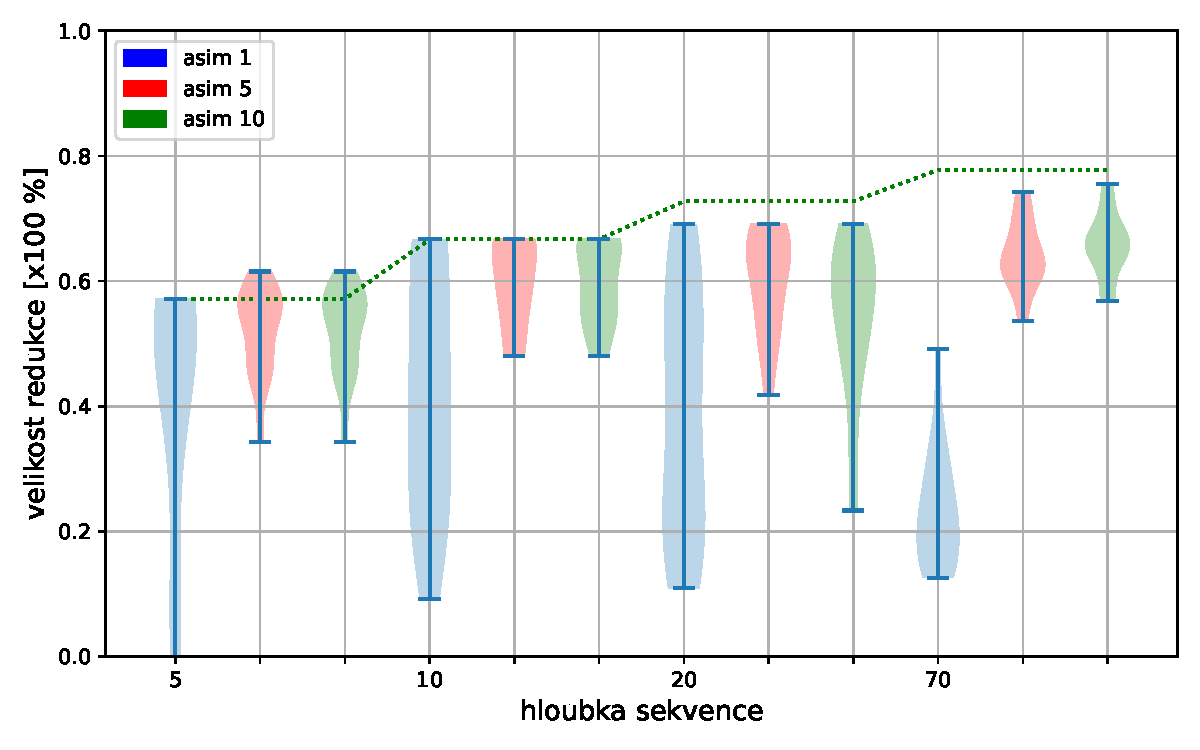
\includegraphics[width=1\linewidth]{5 words: Fork:0.1 Reuse:0.1.pdf}
            \caption{Graf výsledků minimalizace přechodové funkce automatů s následující konfigurací: $in\_cnt = 1$, $fork\_p = 0.1$, $loop\_p = 0.1$, $out\_p = 0$.}
            \label{res2}
        \end{figure}

        \begin{figure}[h]
            \centering
            \captionsetup{justification=justified}
            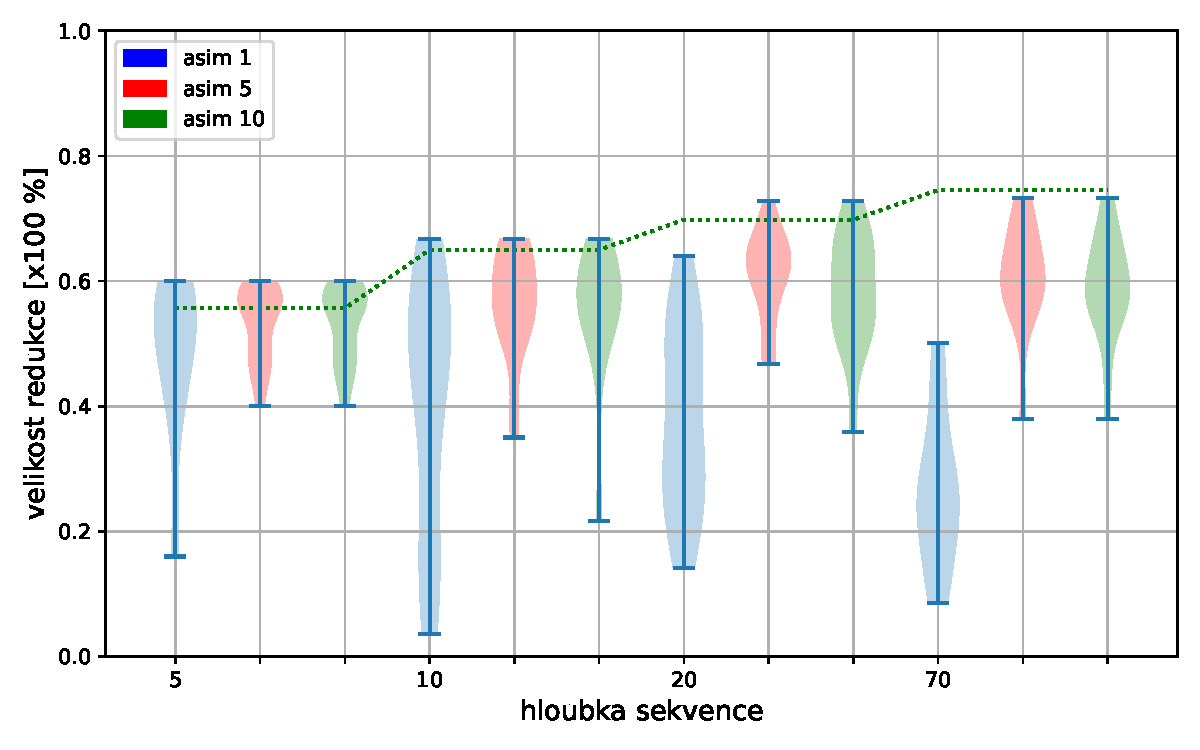
\includegraphics[width=1\linewidth]{5 words: Fork:0.1 Reuse:0.1 Fin:0.05.pdf}
            \caption{Graf výsledků minimalizace přechodové funkce automatů s následující konfigurací: $in\_cnt = 1$, $fork\_p = 0.1$, $loop\_p = 0.1$, $out\_p = 0.05$.}
            \label{res3}
        \end{figure}

        \begin{figure}[h]
            \centering
            \captionsetup{justification=justified}
            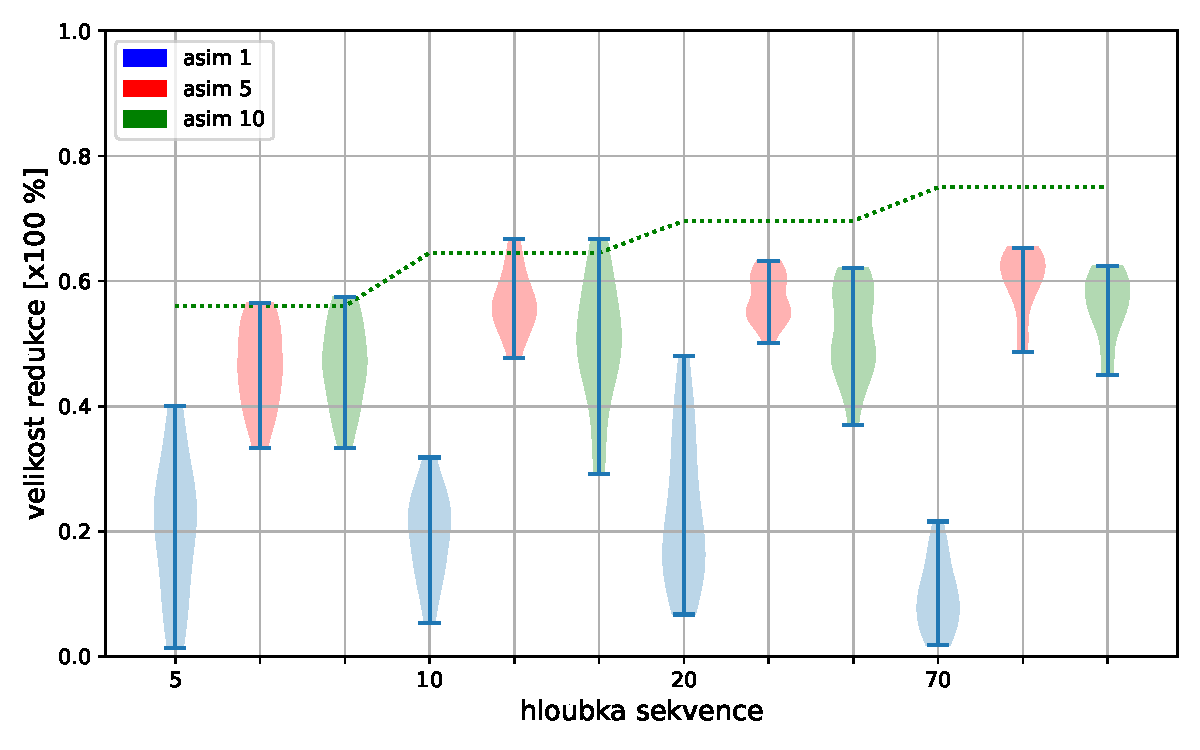
\includegraphics[width=1\linewidth]{5 words: Fork:0.1 Reuse:0.1 Fin:0.05 Init:4.pdf}
            \caption{Graf výsledků minimalizace přechodové funkce automatů s následující konfigurací: $in\_cnt = 4$, $fork\_p = 0.1$, $loop\_p = 0.1$, $out\_p = 0.05$.}
            \label{res4}
        \end{figure}

        \newpage Lze vidět, že se výsledky na obrázcích \ref{res2}, \ref{res3} a~\ref{res4} postupně odchylují od optimálního řešení. Důvodem je složitější struktura automatu, které způsobuje, že sekce reprezentují slova (infixy) různých délek, což znemožňuje plnohodnotně využít relaci $\precapprox$. Tuto situaci lze vidět na obrázku \ref{sufprefBadAtm}. Pro vyřešení tohoto problému je zapotřebí definovat relaci průniku (podobnosti) jazyků.

        \begin{figure}[h]
            \centering
            \captionsetup{justification=justified}
            \begin{tikzpicture}[node distance=1.7cm, every node/.style={font=\footnotesize}]
              \node[state, initial, minimum size=0.5cm] (s) {$s$};
              \node[state, above right of=s, minimum size=0.5cm] (q1) {$q_1$};
              \node[state, below right of=s, minimum size=0.5cm] (q2) {$q_2$};
              \node[state, right of=q1, minimum size=0.5cm] (q3) {$q_3$};
              \node[state, right of=q3, minimum size=0.5cm] (q5) {$q_5$};
              \node[state, right of=q2, minimum size=0.5cm] (q4) {$q_4$};
              \node[state, right of=q4, minimum size=0.5cm] (q6) {$q_6$};
              \node[state, accepting, below right of=q5, minimum size=0.5cm] (f) {$f$};

            \path[->]
                      (s) edge[above left] node{$x$} (q1)
                      (s) edge[below left] node{$y$} (q2)
                      (s) edge[below right, bend right=10] node{$x$} (q3)
                      (s) edge[above right, bend left=10] node{$y$} (q4)
                      (q1) edge[above] node{$a$} (q3)
                      (q3) edge[above] node{$b$} (q5)
                      (q3) edge[below left, bend right=10] node{$x$} (f)
                      (q2) edge[below] node{$a$} (q4)
                      (q4) edge[below] node{$b$} (q6)
                      (q4) edge[above left, bend left=10] node{$y$} (f)
                      (q5) edge[above right] node{$x$} (f)
                      (q6) edge[below right] node{$y$} (f);
            \end{tikzpicture}
            \caption{Příklad automatu přijímajícího slova se stejným prefixem a sufixem, kde jeho složitá struktura znemožňuje použití relace $\precapprox$ pro minimalizaci. Řešením je zavedení relace jazykového průniku.}
            \label{sufprefBadAtm}
          \end{figure}

\section{Závěr}
    Minimalizace velikosti nedeterministických konečných automatů je základní technikou snižující nároky na výpočetní zdroje při operacích s NKA. Dosavadní používané redukční metody, jakými jsou slučování stavů, prořezávání hran přechodů nebo saturace zane-chávají v automatech duplicitní sekvence přechodů. Dokonce existují typy automatů, které tyto algoritmy neumí minimalizovat vůbec.

    V rámci této práce byla zkoumaná nová technika redukce velikosti NKA, využívající vyhledávání po-dobných sekvencí přechodů v automatech a jejich nahrazení jednou "procedurou", která využívá zásobník pro uchování informace o tom, v jaké sekvenci přechodů původního automatu se výpočet nachází. Tato redukční metoda by se dala připodobnit převodu sekvenčního programu na soubor komunikujících procedur.

    Zkoumaný minimalizační algoritmus byl testován na 960 (za tímto účelem vygenerovaných) automatech. Při použití relace \textit{aproxsim} do vzdálenosti 10 přechodů od zkoumaných stavů se míra redukce blížila maximální možné teoretické hranici. Pro zvýšení míry redukce by bylo nutné použít relaci jazykového průniku (podobnosti jazyků).

\section{Budoucí práce}
    Jak již bylo zmíněno, pro vylepšení minimalizačního algoritmu založeného na vyhledávání procedur je po-třeba definovat relaci jazykové podobnosti. Tato relace musí nejenom udávat průnik jazyků zkoumaných stavů, ale také musí určovat teoretický možný počet ušetře-ných přechodů, kterého by bylo dosaženo při nahrazení těchto stavů a jejich následníků procedurou.

\section{Poděkování}
    Děkuji svému vedoucímu doc. Mgr. Lukáši Holíkovi, Ph.D za jeho podporu a čas, který mne věnoval při práci na tomto výzkumu.